%%
%% Copyright 2022 OXFORD UNIVERSITY PRESS
%%
%% This file is part of the 'oup-authoring-template Bundle'.
%% ---------------------------------------------
%%
%% It may be distributed under the conditions of the LaTeX Project Public
%% License, either version 1.2 of this license or (at your option) any
%% later version.  The latest version of this license is in
%%    http://www.latex-project.org/lppl.txt
%% and version 1.2 or later is part of all distributions of LaTeX
%% version 1999/12/01 or later.
%%
%% The list of all files belonging to the 'oup-authoring-template Bundle' is
%% given in the file `manifest.txt'.
%%
%% Template article for OXFORD UNIVERSITY PRESS's document class `oup-authoring-template'
%% with bibliographic references
%%

%%%CONTEMPORARY%%%
\documentclass[unnumsec,webpdf,contemporary,large]{oup-authoring-template}%
%\documentclass[unnumsec,webpdf,contemporary,large,namedate]{oup-authoring-template}% uncomment this line for author year citations and comment the above
%\documentclass[unnumsec,webpdf,contemporary,medium]{oup-authoring-template}
%\documentclass[unnumsec,webpdf,contemporary,small]{oup-authoring-template}

%%%MODERN%%%
%\documentclass[unnumsec,webpdf,modern,large]{oup-authoring-template}
%\documentclass[unnumsec,webpdf,modern,large,namedate]{oup-authoring-template}% uncomment this line for author year citations and comment the above
%\documentclass[unnumsec,webpdf,modern,medium]{oup-authoring-template}
%\documentclass[unnumsec,webpdf,modern,small]{oup-authoring-template}

%%%TRADITIONAL%%%
%\documentclass[unnumsec,webpdf,traditional,large]{oup-authoring-template}
%\documentclass[unnumsec,webpdf,traditional,large,namedate]{oup-authoring-template}% uncomment this line for author year citations and comment the above
%\documentclass[unnumsec,namedate,webpdf,traditional,medium]{oup-authoring-template}
%\documentclass[namedate,webpdf,traditional,small]{oup-authoring-template}

%\onecolumn % for one column layouts

%\usepackage{showframe}

\graphicspath{{Fig/}}

% line numbers
%\usepackage[mathlines, switch]{lineno}
%\usepackage[right]{lineno}

\theoremstyle{thmstyleone}%
\newtheorem{theorem}{Theorem}%  meant for continuous numbers
%%\newtheorem{theorem}{Theorem}[section]% meant for sectionwise numbers
%% optional argument [theorem] produces theorem numbering sequence instead of independent numbers for Proposition
\newtheorem{proposition}[theorem]{Proposition}%
%%\newtheorem{proposition}{Proposition}% to get separate numbers for theorem and proposition etc.
\theoremstyle{thmstyletwo}%
\newtheorem{example}{Example}%
\newtheorem{remark}{Remark}%
\theoremstyle{thmstylethree}%
\newtheorem{definition}{Definition}

\usepackage[normalem]{ulem}

\begin{document}

\sloppy

\journaltitle{Journal Title Here}
\DOI{DOI HERE}
\copyrightyear{2022}
\pubyear{2019}
\access{Advance Access Publication Date: Day Month Year}
\appnotes{Paper}

\firstpage{1}

%\subtitle{Subject Section}


\title[MsQuality: Calculation of standardized quality metrics of mass spectrometry data]{MsQuality – an interoperable open-source package for the calculation of standardized quality metrics of mass spectrometry data}

%\author[1,$\ast$]{Thomas Naake}
%\author[2]{Johannes Rainer}
%\author[1]{Wolfgang Huber}


\author[Naake \textit{et~al}.]{Thomas Naake\,$^{\text{\sfb 1}}$, Johannes Rainer,$^{\text{\sfb 2}}$ and Wolfgang Huber\,$^{\text{\sfb 1}*}$}



%\authormark{Naake et al.}

\address{
$^{\text{\sf 1}}$ Genome Biology Unit, European Molecular Biology Laboratory, Heidelberg, 69117, Germany \\
$^{\text{\sf 2}}$ Institute for Biomedicine (Affiliated to the University of L\"ubeck), Eurac Research, Viale Druso 1, 39100 Bolzano, Italy}

\corresp{$^\ast$corresponding author.  \href{email:wolfgang.huber@embl.org}{wolfgang.huber@embl.org}}



\received{Date}{0}{Year}
\revised{Date}{0}{Year}
\accepted{Date}{0}{Year}

%\editor{Associate Editor: Name}

%\abstract{
%\textbf{Motivation:} .\\
%\textbf{Results:} .\\
%\textbf{Availability:} .\\
%\textbf{Contact:} \href{name@email.com}{name@email.com}\\
%\textbf{Supplementary information:} Supplementary data are available at \textit{Journal Name}
%online.}

\abstract{
\textbf{Motivation:} Multiple factors can impact accuracy and reproducibility
of mass spectrometry data. There is a need to integrate quality
assessment and control into data analytic workflows. \\
\textbf{Results:} The \texttt{MsQuality} package calculates 
\textcolor{red}{\sout{40}}\textcolor{red}{43} low-level quality metrics based
 on the controlled mzQC vocabulary defined by the HUPO-PSI on a single
mass spectrometry-based
measurement of a sample. It helps to identify low-quality measurements and 
track data quality.  Its use of community-standard quality metrics facilitates
comparability of
quality assessment and control (QA/QC) criteria across datasets.\\
\textbf{Availability:} The R package \texttt{MsQuality} is available through 
Bioconductor at https://bioconductor.org/packages/MsQuality.\\
\textbf{Contact:} \href{naake@embl.de}{naake@embl.de}\\
\textbf{Supplementary information:} Supplementary data are available at \textit{Bioinformatics}
online.}
\keywords{quality control, mass spectrometry, metabolomics, proteomics, R}

% \boxedtext{
% \begin{itemize}
% \item Key boxed text here.
% \item Key boxed text here.
% \item Key boxed text here.
% \end{itemize}}

\maketitle

Mass spectrometry (MS) is a versatile analytical technique that has been adopted
in a variety of disciplines, including proteomics, metabolomics, and lipidomics, 
enabling the identification and quantification of a wide range of molecules. 
Obtaining high-quality data from mass spectrometry experiments can be a 
challenging task, as numerous factors can impact the accuracy and 
reproducibility of the obtained data. To ensure that MS data is fit for purpose, 
quality assessment and quality control (QA/QC) need to be performed close
to data production from raw data \citep{Koecher2011,Bereman2015}. 
Use of standardized quality metrics described by a controlled vocabulary helps in making QA/QC more 
comparable across datasets and data producers and increases transparency and 
trustworthiness of such measures as viewed by data users 
\citep{Mayer2012,Mayer2013}. 

Here, we introduce the \texttt{MsQuality} R \textcolor{red}{\sout{-} }package, which provides 
functionality to calculate, assess, and track quality metrics for mass 
spectrometry-derived spectral data of a single mass-spectrometry-based 
measurement of a sample. 
The package provides \textcolor{red}{\sout{40}}\textcolor{red}{43} of the mzQC quality metrics defined by
the Human Proteome Organization-Proteomics Standards Initiative (HUPO-PSI,
hupo-psi.github.io/mzQC). 
\textcolor{red}{Its use of community standards for data
representation in mass spectrometry defined by HUPO-PSI facilitates comparison, 
consistent
storage, reporting and exchange of quality metrics and quality control criteria.}
The \textcolor{red}{\sout{se}}\textcolor{red}{metrics} are calculated on low-level MS data
such as retention times, $m/z$, and associated intensity values.
The package automates tracking and quantification of data quality 
\textcolor{red}{on a per-measurememt basis} and 
helps to integrate these computations in routine workflows, thereby,
\texttt{MsQuality} facilitates the identification of measurements \textcolor{red}{\sout{with low 
quality, including those}} with a high occurrence of missing values, 
ahead-of-time termination of chromatographic runs, \textcolor{red}{\sout{or}} low instrument sensitivity,
\textcolor{red}{variations in calibration, and batch and confounding 
effects within datasets (Fig. \ref{fig:fig1} a and b)}. 

Following the definitions by \cite{Bittremieux2017}, \texttt{MsQuality}
focuses on the calculation of inter-experiment metrics, which is a
summarization of an intra-experiment metric. Examples for
intra-experiment metrics are the chromatogram of the total ion current (TIC) 
over the retention time. Inter-experiment metrics, on the other hand, 
facilitate the comparison of multiple MS runs or experiments, 
e.g., via longitudinal analysis of quality metrics, such as the
fractions of the total retention time required to accumulate a given
percentile of the TIC.

\section{Usage scenario and implementation} \label{usagescenario}

\textcolor{red}{\sout{\texttt{MsQuality} offers easy-to-use means of evaluating data quality on a
per-measurement basis, including the identification of low-quality measurements,
biases and outliers, variations in calibration, and batch and confounding effects within
datasets (Fig. \ref{fig:fig1} a and b). }}
\textcolor{red}{\sout{Its use of community standards for data
representation in mass spectrometry defined by HUPO-PSI facilitates comparison, 
consistent
storage, reporting and exchange of quality metrics and quality control criteria.}}

\begin{figure}
    \centering
 	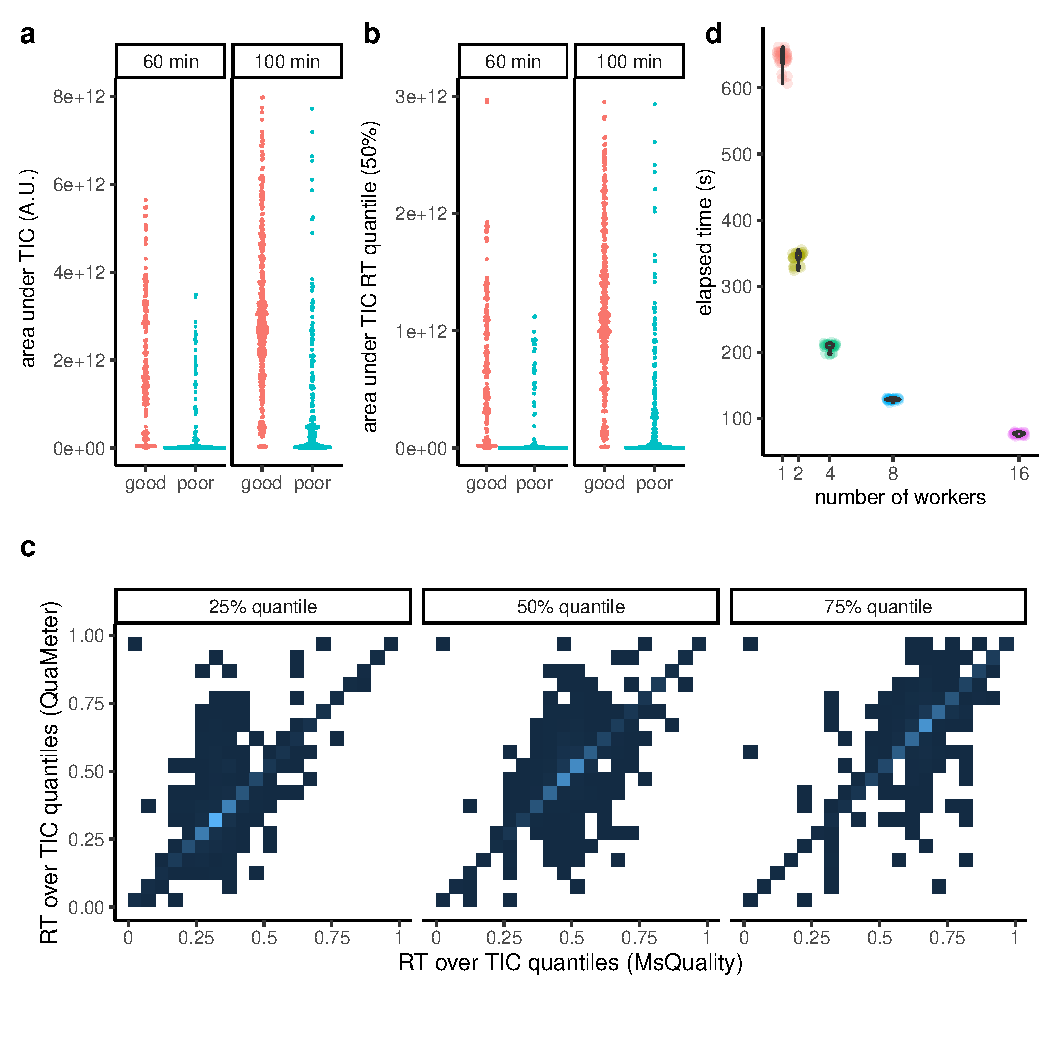
\includegraphics[scale=0.51, clip, trim=0 37 0 5, scale = 0.9]{figure-main}
 	  \caption{Examples of \texttt{MsQuality} functionality. Metrics are based
 	        on MS1 spectra; one data point is obtained per MS1 spectrum.
 	        (a) Area under TIC: The area under the total ion chromatogram. 
            (b) Quantiles of area under the total ion
                chromatogram of the retention time (TIC RT), here, the 50\% quantile. 
  	      For (a) and (b) the data points are displayed \textcolor{red}{as log-values}
                in a beeswarm plot and stratified for high-quality and low-quality
                measurements as classified in \cite{Amidan2014}.
            (c) Comparison of quality metrics calculated by \texttt{MsQuality} 
                and \texttt{QuaMeter}: RT over \textcolor{red}{\sout{TIC quantiles}}
		\textcolor{red}{MS quarters}. The
	      data points are displayed as 2D densities. Brighter areas corresond to
               high 2D density areas.
            (d) Wall-clock execution time for the calculation of quality metrics of the 
                data set of \cite{Amidan2014} when parallel computing is used 
                (1, 2, 4, 8, and 16 workers). A.U. arbitrary units.
    } \label{fig:fig1}
\end{figure}

The versatility of \texttt{MsQuality} in calculating metrics extends to a wide range of
applications, from small-scale studies to long-term acquisition of mass spectrometry
data, e.g. a core facility running an instrument for months and years. 
We demonstrate the utility of \texttt{MsQuality} in two case studies: a 
\textcolor{red}{metabolomics}
dataset of 180 cancer cell lines obtained by flow injection analysis
\citep{Cherkaoui2022} and a \textcolor{red}{proteomics} liquid chromatography
 (LC)-MS dataset of the same 
control sample \citep{Amidan2014} as instance of a long-term quality control 
usage scenario. 

The values computed by \texttt{MsQuality}
agree with those of \texttt{QuaMeter} \citep{Ma2012} (Fig. \ref{fig:fig1} c): 
\textcolor{red}{after removing zero-length and zero-intensity entries, as is done by \texttt{QuaMeter},}
75\% of the \textcolor{red}{\sout{analyzed \texttt{MsQuality}} 20 compared} metrics showed Pearson correlation 
coefficients over \textcolor{red}{\sout{0.81} 0.98} and Spearman correlation coefficients 
over \textcolor{red}{\sout{0.87} 0.99} (see the Supplementary Data for further details).

\textcolor{red}{Previously developed QC software, such as \texttt{PTXQC} \citep{Bielow2016}, 
\texttt{pmultiqc} \citep{Riverol2023}, \texttt{QCloud2} \citep{Olivella2021}, and \texttt{QuaMeter}, 
focused their calculation of QC metrics on proteomics data. \texttt{MsQuality}, on the other hand, is 
agnostic towards the underlying technology (e.g., proteomics, metabolomics, lipidomics).}
It is implemented as an GPL-3-licensed open-source R package, 
\textcolor{red}{and integrates seamlessly into the 
\texttt{RforMassSpectrometry}/Bioconductor infrastructure for MS data analysis.}
\textcolor{red}{The package builds} \textcolor{red}{\sout{building}} 
upon the established \texttt{Spectra} and \texttt{MsExperiment} packages
\citep{Rainer2022} to provide and represent the MS data. Thus, \texttt{MsQuality} 
supports a large variety of data input formats
\textcolor{red}{(ranging from mzML, mzXML, CDF, MGF, MSP to some raw vendor 
file formats, such as Bruker TimsTOF and Thermo raw files)}
as well as analyses of very large experiments through the use of data
representations with low memory footprint. 
\textcolor{red}{As \texttt{MsQuality} is written in the software environment R for statistical computing, it facilitates 
automatized, scalable, easy-to-archive, and shareable scripts for complete 
data analysis workflows, including pre-processing and statistical analysis steps.}
Native parallelization enables a fast
and scalable calculation of quality metrics (Fig. \ref{fig:fig1} d, 
see the Supplementary Data for further details).

\textcolor{red}{Besides the human-readable output of quality metrics as a data frame, 
\texttt{MsQuality} enables the users to export the metrics via the mzQC-defined reporting 
and exchange file format via the \texttt{rmzqc} package \citep{Bielow2023}.}
Finally, \texttt{MsQuality} requires little programmatic interaction and is designed to be
user-friendly\textcolor{red}{\sout{.}}\textcolor{red}{: (i)}  after the instantiation of 
\texttt{Spectra} or \texttt{MsExperiment}
object, a single function call is needed to calculate the quality metrics\textcolor{red}{\sout{.}} 
\textcolor{red}{; (ii) the metrics can be interactively explored via a shiny application}.


\section{Conclusion}

The \texttt{MsQuality} R \textcolor{red}{\sout{-} }package provides functionality to calculate, assess, 
and track quality metrics for mass spectrometry-derived spectral data. 
It offers easy-to-use means of evaluating data quality \textcolor{red}{\sout{on a per-measurement 
basis}}, enabling researchers the identification of low-quality measurements.
By using standardized quality metrics via the controlled vocabulary of HUPO-PSI,
\texttt{MsQuality} helps to make QA/QC more comparable across datasets and 
data producers.
The implementation of \texttt{MsQuality}'s metric calculation is designed
to be user-friendly and streamlined and requires little programmatic 
interaction, facilitating reproducible calculation and evaluation of data 
quality metrics.
\texttt{MsQuality} contributes to the expanding list of 
tools that use the \texttt{Spectra}/\texttt{MsExperiment} framework 
\citep{Rainer2022} to address various stages in the analysis pipeline of 
mass spectrometry data. By building upon this extensive ecosystem for 
mass spectrometry data, 
\texttt{MsQuality} enables researchers to create seamless analysis workflows 
for rapid, efficient, and standardized evaluation of MS data quality, 
ultimately leading to more robust scientific discoveries in mass spectrometry
workflows.


\section{Acknowledgements}

We acknowledge feedback from Friedemann Ringwald, Hagen Gegner, and 
Torsten M\"uller on usability of 
\texttt{MsQuality} and all developers and maintainers of the R/Bioconductor 
packages \texttt{MsQuality} is built upon. We would like to thank Nicola Zamboni
for his valuable assistance in locating and understanding the data of 
\citet{Cherkaoui2022}. 

\subsection{Author contributions statement}

T.N. conceptualized the project. T.N. and J.R. implemented the algorithms as 
an R package. T.N. analysed the results. W.H. provided feedback and guidance. 
T.N., J.R. and W.H. wrote the manuscript.



\subsection{Funding}

This work was supported by the Bundesministerium für Bildung und Forschung 
[grant agreement no. 161L0212E].

Conflict of Interest: none declared.


%\bibliographystyle{plain}
%\bibliography{reference}

\begin{thebibliography}{10}
\bibitem[Amidan \textit{et~al}., 2014]{Amidan2014}
Amidan, B.G. \textit{et~al}. (2014) Signatures for mass spectrometry data
quality.
\textit{Proteome Research}, \textbf{13}, 2215--2222.

\bibitem[Bereman, 2015]{Bereman2015}
Bereman, M.S. (2015) Tools for Monitoring System Suitability in LC MS/MS
Centric Proteomic Experiments.
\textit{Proteomics}, \textbf{15}, 891--902.

\bibitem[Bielow \textit{et~al}., 2016]{Bielow2016}
Bielow, C. \textit{et~al}., M.S. (2016) Proteomics Quality Control: Quality 
Control Software for MaxQuant Results.
\textit{Proteome Research}, \textbf{15}, 777--787.

\bibitem[Bielow, 2023]{Bielow2023}
Bielow, C. (2023) rmzqc: Creation, Reading and Validation of 'mzqc' Files,
R package version 0.5.1, available via 
https://CRAN.R-project.org/package=rmzqc.

\bibitem[Bittremieux \textit{et~al}., 2017]{Bittremieux2017}
Bittremieux, W. \textit{et~al}. (2017) Computational quality control tools for
mass spectrometry proteomics.
\textit{Proteomics}, \textbf{17}, 1--11.

\bibitem[Cherkaoui \textit{et~al}., 2022]{Cherkaoui2022}
Cherkaoui, S. \textit{et~al}. (2022) A functional analysis of 180 cancer cell
lines reveals conserved intrinsic metabolic programs.
\textit{Molecular Systems Biology}, \textbf{18}, e11033.

\bibitem[K\"ocher \textit{et~al}., 2011]{Koecher2011}
K\"ocher, T. \textit{et~al}. (2011) Quality control in LC-MS/MS.
\textit{Proteomics and Systems Biology}, \textbf{11}, 1026--1030.

% \bibitem[Paulovich \textit{et~al}., 2010]{Paulovich2010}
% Paulovich, A.G. \textit{et~al} (2010) Interlaboratory Study Characterizing a 
% Yeast Performance Standard for Benchmarking LC-MS Platform Performance.
% \textit{Molecular \& Cellular Proteomics}, \textbf{9}, 242--254.

\bibitem[Ma \textit{et~al}., 2012]{Ma2012}
Ma, Z.-Q. \textit{et~al} (2012) QuaMeter: Multivendor Performance Metrics
for LC–MS/MS Proteomics Instrumentation.
\textit{Analytical Chemistry}, \textbf{84}, 5845--5850.

\bibitem[Mayer \textit{et~al}., 2012]{Mayer2012}
Mayer, G. \textit{et~al} (2012) Controlled vocabularies and ontologies in 
proteomics: overview, principles and practice.
\textit{Biochim Biophys Acta}, \textbf{1844}, 98--107.

\bibitem[Mayer \textit{et~al}., 2013]{Mayer2013}
Mayer, G. \textit{et~al} (2013) The HUPO proteomics standards initiative - 
mass spectrometry controlled vocabulary.
\textit{Database}, \textbf{2013}, bat009.

\bibitem[Olivella \textit{et~al}., 2021]{Olivella2021}
Olivella, R. \textit{et~al} (2021) QCloud2: An Improved Cloud-based 
Quality-Control System for Mass-Spectrometry-based Proteomics Laboratories.
\textit{Proteome Research}, \textbf{2021}, 20210--2013.

% \bibitem[Naake \textit{et~al}., 2022]{Naake2022}
% Naake, T. \textit{et~al} (2022) MatrixQCvis: shiny-based interactive data
% quality exploration for omics data.
% \textit{Bioinformatics}, \textbf{38}, 1181--1182.

\bibitem[Rainer \textit{et~al}., 2022]{Rainer2022}
Rainer, J. \textit{et~al} (2022) A Modular and Expandable Ecosystem for Metabolomics Data Annotation in R.
\textit{Metabolites}, \textbf{12}, 173.

\bibitem[Riverol \textit{et~al}., 2023]{Riverol2023}
Perez-Riverol, Y. \textit{et~al} (2023) nf-core/quantms: nf-core/quantms v1.1.0 - Berlin-Bern (1.1.1).
\textit{Zenodo}, https://doi.org/10.5281/zenodo.7774139.

\end{thebibliography}


%USE THE BELOW OPTIONS IN CASE YOU NEED AUTHOR YEAR FORMAT.
%\bibliographystyle{abbrvnat}
%\bibliography{reference}



\end{document}
